\documentclass{whutmod}
\usepackage[linesnumbered,ruled,lined]{algorithm2e}
\bibliographystyle{unsrt}
\team{10}
\membera{刘子川}
\joba{编程}
\memberb{程宇}
\jobb{建模}
\memberc{祁成}
\jobc{写作}
\hypersetup{
	colorlinks=true,
	linkcolor=black,citecolor=black
}


\newcommand{\upcite}[1]{\textsuperscript{\cite{#1}}}
%%%%%%%%%%%%%%%%%%%%%%%%%%%%%%%%%题目%%%%%%%%%%%%%%%%%%%%%%%%%%%%%%%%%%%%
\title{基于xxxxxxxx模型}
\tihao{1} 

\begin{document}

	\maketitle
	\thispagestyle{empty}
%%%%%%%%%%%%%%%%%%%%%%%%%%%%%%%%%摘要%%%%%%%%%%%%%%%%%%%%%%%%%%%%%%%%%%%%
	\begin{abstract}
		控制高压油管的压力变化对减小燃油量偏差,提高发动机工作效率具有重要意义。本文建立了基于质量守恒定理的微分方程稳压模型,采用二分法、试探法以及自适应权重的蝙蝠算法对模型进行求解。
		//
	
		针对问题一,建立基于质量守恒定律的燃油流动模型,考察单向阀开启时间对压力稳定性的影响。综合考虑压力与弹性模量、密度之间的关系,提出燃油压力-密度微分方程模型和燃油流动方程。本文采用改进的欧拉方法对燃油压力-密度微分方程求得数值解;利用二分法求解压力分布。综合考虑平均绝对偏差等反映压力稳定程度的统计量,求得直接稳定于100MPa的开启时长为\textbf{0.2955ms} ,在2s、5s内到达并稳定于150MPa时开启时长为\textbf{0.7795ms}、\textbf{0.6734ms},10s到达并稳定于150MPa的开启时长存在多解。最后对求解结果进行灵敏度分析、误差分析。
		//
	
		针对问题二,建立基于质量守恒定律的泵-管-嘴系统动态稳压模型,将燃油进入和喷出的过程动态化处理。考虑柱塞和针阀升程的动态变动,建立喷油嘴流量方程和质量守恒方程。为提高角速度求解精度,以凸轮转动角度为固定步长,转动时间变动步长,采用试探法粗略搜索与二分法精细搜索的方法求解,求得凸轮最优转动角速度\textbf{0.0283rad/ms(转速270.382转/分钟)},并得到该角速度下高压油管的密度、压力周期性变化图。对求解结果进行误差分析与灵敏度分析,考察柱塞腔残余容积变动对高压油管压力稳态的影响。
		//
	
		针对问题三,对于增加一个喷油嘴的情况,改变质量守恒方程并沿用问题二的模型调整供、喷油策略,得到最优凸轮转动角速度为\textbf{0.0522rad/ms(498.726转/分钟)};对于既增加喷油嘴又增加减压阀的情况,建立基于自适应权重的蝙蝠算法的多变量优化模型,以凸轮转动角速度、减压阀开启时长和关闭时长为参数,平均绝对偏差MAD为目标,在泵-管-嘴系统动态稳压模型的基础上进行求解,得到最优参数:\textbf{角速度0.0648 rad/ms(619.109转/分钟)}、减压阀的开启时长\textbf{2.4ms}和减压阀的关闭时长\textbf{97.6ms}。
		//
	
		本文的优点为:1. 采用试探法粗略搜索与二分法精细搜索结合的方法,降低了问题的求解难度。2.以凸轮转动角度为固定步长,对不同角速度按照不同精度的时间步长求解,大大提高了求解的精确度。 3.针对智能算法求解精度方面,采用改进的蝙蝠算法,使速度权重系数自适应调整,兼顾局部搜索与全局搜索能力。
		
		\keywords{
			微分方程\quad
			微分方程\quad	
			微分方程\quad
			微分方程\quad
		}
	\end{abstract}


%%%%%%%%%%%%%%%%%%%%%%%%%%%%%%%%%目录%%%%%%%%%%%%%%%%%%%%%%%%%%%%%%%%%%%%
	\thispagestyle{empty}
	\tableofcontents
	\setcounter{page}{0}                                               
	\newpage	%换页符
	

	
	\section{问题重述}	
		\subsection{问题背景}
%	    	分析研究\upcite{1}。xxxxxxxxxxx\footnote{\quad xxxxxxxxxx.}.
	
自动指纹识别系统(automated fingerprint identification system,简称 AFIS)有着广泛的应用背景。目前对自动 指纹识别系统的研究主要有 3 个方面,即图像增强、指纹分类和细节匹配。一般可以分成"离线部分"和"在线部分"两个部分。如图 \ref{lssct} 所示,离线部分包括用指纹采集仪采集指纹、提取出细节点、将细节点保存到数据库中形成指纹模板库等主要步骤。在线部分包括用指纹采集仪采集指纹、提取出细节点、然后将这些细节点与保存在数据库中模板细节点进行匹配,判断输入细节点与模板细节点是否来自同一个手指的指纹\upcite{1,3}。指纹分类一般是用在大规模的指纹库中,作为细节匹配中减少搜索范围的步骤使用。指纹图像一般占用较多的空间,且图像中的像素信息并不适合计算机进行分析或匹配。为实现计算机自动识别,需要有一种方法来描述指纹的内在结构、具体形态和其它特征并将其用最少的字节数来存储于计算机中。此计算机系统可扫描犯罪现场采集的指纹,并且与州、地区、国家之间执法机关采集的数百万指纹档案互相比对\upcite{2}。指纹由专家追踪后,经计算机扫描,得到许多细节来和数据库里其它指纹比对,列出相符合的百分比来让鉴识人员得知可能的相符人选\footnote{\quad https://baike.baidu.com/item/AFIS/2851410?fr=aladdin}。任何计算机比对的结果,都会经指纹专家比较与此指纹相关的样本来验证。
				\begin{figure}[H]
	\centering
	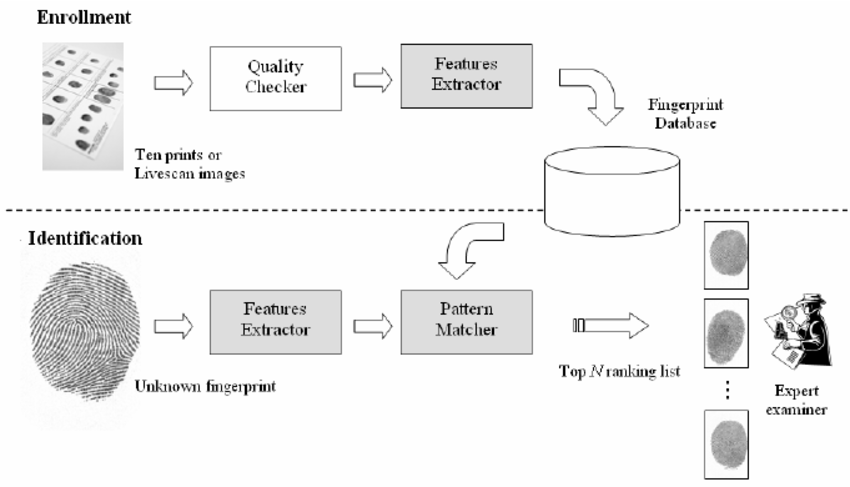
\includegraphics[width=.8\textwidth]{figures/AFIS.png}
	\caption{自动指纹识别系统框图 }\label{lssct}
\end{figure}

		\subsection{问题概述}
		    围绕相关附件和条件要求,试根据附件中的16幅指纹图像,不借助现有的指纹相关软件,依次提出以下问题:
				 
			
			\textbf{编码:} 给出一种用不超过200字节(下面称为“指纹密码”)来刻画描述指纹基本特征的表示方法,介绍其数学原理。
			
			\textbf{匹配:} 将你的方法编程实现,对附件中的每一幅指纹都给出其“指纹密码”的表示。基于你找到的这些指纹表示,你能否给出一种方法比较不同指纹间的异同及相似程度?
			
			\textbf{应用:} 你能否对附件中的16个指纹进行对比和归类?请给出你对比及分类的依据和结果。

	\section{模型假设}
		\begin{itemize}                                             
		\item [(1)] 
		\item [(2)]
		\item [(3)] 
		\item [(4)] 
		\end{itemize}

		
	\section{符号说明}
		\begin{table}[H]
		\centering
		\setlength{\tabcolsep}{12mm}
		\begin{tabular}{cc}
			\toprule[1.5pt]
			\multicolumn{1}{m{5cm}}{\centering 符号} & \multicolumn{1}{m{5cm}}{\centering 说明} \\
			\midrule[1pt]		
			$P_n$  & 20个站点  \\ 
			$P_n$  & 20个站点  \\ 
		   	$P_n$  & 20个站点  \\ 
			\bottomrule[1.5pt]
		\end{tabular}
		\begin{tablenotes}
		\item 注:表中未说明的符号以首次出现处为准
		\end{tablenotes}
		\end{table}

	\section{问题一模型的建立与求解}
		\subsection{问题描述与分析}
			问题一要求给出一种用不超过200字节来刻画描述指纹基本特征的表示方法。传统的图像压缩方法有霍夫曼压缩、Golomb编码、LZW编码、小波编码等,这些都能对指纹进行刻画。但是相对于200字节的限制而言,他们在压缩编码方向显得不敬人意。
			
			相较于传统的图片编码而言,通过网络编码能更有效的提高图像在细节上的依赖。在网络训练的过程中,网络只用到该向量之中少量元素,其中的大部分元素对于网络来说是没有用的。自编码器通过无监督学习来提取有用的信息,对于手写数字图片来说可能是颜色为黑色的像素点,将图片中的很大一部分白色像素舍弃,只提取对网络有用的信息,到达降低数据维度的目的,从而实现小样本编码。
		
%			其思维流程图如图~\ref{lct}~所示:
%			\begin{figure}[H]
%				\centering
%				
\includegraphics[width=\textwidth]{figures/whut.jpg}
%				\caption{问题一思维流程图}\label{lct}
%			\end{figure}
%			
		\subsection{搭建卷积自编码器模型}
		   自编码器(AutoEncoder)是一种能够通过无监督学习,学到输入数据高效表示的人工神经网络。输入数据的这一高效表示称为编码(codings),其维度一般远小于输入数据,使得自编码器可用于降维。更重要的是,自编码器可作为强大的特征检测器(feature detectors),应用于深度神经网络的预训练。我们以VGG模型\upcite{4}结构为基础,构造一个 新的卷积神经网络模型,并通过交叉验证的思想训练小样本数据,调整
		   模型参数,得到小样本条件下最优的卷积神经网络模型。
		
			\subsubsection{卷积神经网络}
			
			\paragraph{Convolution Kernel} 在图像处理的过程中,我们经常会用到矩阵卷积来计算图像(image)的特征(feature),矩阵卷积有两种:全卷积(full convolution)和有效值卷积(valid convolution),其全卷积核函数的定义式为:
			     \begin{gather}
z(u, v)=\sum_{i=-\infty}^{\infty} \sum_{j=-\infty}^{\infty} x_{i, j} \cdot k_{u-i, v-j},
			     \end{gather}
			有效值卷积的定义式为:
			\begin{gather}
\begin{array}{c}
z(u, v)=\sum_{i=-\infty}^{\infty} \sum_{j=-\infty}^{\infty} x_{i+u, j+v} \cdot k_{r o t i, j} \cdot \chi(i, j) \\
\chi(i, j)=\left\{  
\begin{array}{c}
1,0 \leqslant i, j \leqslant n \\
0, \text {others}
\end{array}
\right.  
\end{array},
			\end{gather}
			其中$X$是灰度图像转换为$m\times m$阶矩阵,$K$是$n\times n$阶卷积核,一般取$3\times 3$,$K_{rot}$是由$K$转置得到。
			
		那么,从 Input Image 到 Output Image 的变化如下图所示:
		\begin{figure}[H]
			\centering
			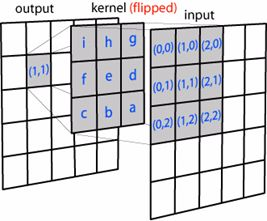
\includegraphics[width=.5\textwidth]{figures/cnn.jpg}
			\caption{卷积核函数示意图}
		\end{figure}
		可以看出,其实二维卷积一样也是加权叠加/积分。需要注意的是,其中 Convolution Kernel 进行了水平和竖直方向的翻转。
		
			\paragraph{Pooling} 对于灰度图像的采样而言,Pooling 对于输入的 Feature Map,选择某种方式对其进行压缩。如下图,表示的就是对$2\times 2$邻域内的值,选择最大值输出到下一层,这叫做 Max-Pooling。
				\begin{figure}[H]
			\centering
			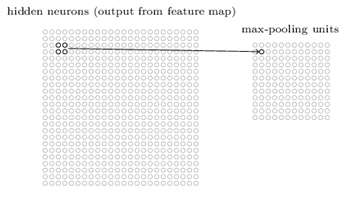
\includegraphics[width=.5\textwidth]{figures/pool.png}
			\caption{池化层Max-Pooling示意图}
		\end{figure}
	
	对卷积层进行池化从而通过对 Feature Map 降维,有效减少后续层需要的参数,当其中像素在邻域发生微小位移时,Pooling Layer 的输出是不变的。这就增强了网络的鲁棒性,有一定抗扰动的作用。
	
	\paragraph{Activation} 激活层的正向传播主要依靠众多神经元的计算来完成的,工作过程中可以用下式来表示:
	\begin{gather*}
	{u_{k}=\sum_{i=1} w_{k i} x_{i}}, \\ {y_{k}=f\left(u_{k}-b_{k}\right)},
	\end{gather*}
	其中:$x_{i}$表示第 i 个输入; $w_{ki}$表示与第 i 输入量相连的权值;$u_{k}$表示所有输入的加权和;$b_{k}$为神经 元阈值;$ f$ 为激活函数;$y_{k}$ 为神经网络的输出。
	
	激活函数的种类有很多,如 $sigmoid$, $tanh$ 及$ Relu$,本文应用的是 $Relu$作为激活函数搭建两层隐含层,如式~\ref{shiw}~所示:
	\begin{gather}\label{shiw}
	\begin{array}{c}{f_{\text {Relu}}=\max (0, z)}\\
	\frac{d}{d z} f_{R e L U}=\left\{\begin{array}{ll}{1,} & {z>0} \\ {0,} & {z \leqslant 0}\end{array}\right.
	\end{array}.
	\end{gather}
	
	网络的输出层使用$ softmax $函数作分类器, 式~\ref{shiq}~为第 i 个神经的输出:
	\begin{gather*}\label{shiq}
	f_{\text {softmax}}=\mathrm{e}^{i} / \sum_{j} \mathrm{e}^{j}.
	\end{gather*}
	
			\subsubsection{卷积自动编码器}
			普通的自编码器中,编码器和解码器中层与层之间的连
			接方式为全连接,该编码器具有一个输入层,n个隐藏层和一个输出层,
			
			给定图片样本$X=\left\{ x_1,x_2,\cdots,x_nx \right\}, X\in \mathbb{R}^{n\times c\times w \times h}$,其中c为通道数。自编码器首先将$x_i$编码成$y(x_i)$再解码成$z(y_i)$,其公式L表述如下:
				\begin{gather}
			\begin{array}{l}
			y(x)=Encoder\left(W_{1} x+b\right) \\
			z(x)=Decoder\left(W_{2} y(x)+c\right)
			\end{array}.
			\end{gather}
			
			通过最小化重建误差$L(X,Z)$,我们可以获得模型参数,这里用θ表示为:
			\begin{gather}
			\theta=\underset{\theta}{\arg \min } L(X, Z)=\underset{\theta}{\arg \min } \frac{1}{2} \sum_{i=1}^{N}\left\|x^{(i)}-z\left(x^{(i)}\right)\right\|^{2}.
			\end{gather}

			本文卷积自编码器(ConvAutoEncoder, CAE)中的编码器部分的网络结构与卷积神
			经网络中卷积池化部分的结构相同。首先通过编码器部分构
			造出对应的解码器部分,在训练结束后,保留编码器部分的结
			构和权重,在编码器后加上与卷积神经网络结构中相同的全
			连接层来进行图像的编码与分类识别。其卷积自编码器$L(X,Z)$的具体结构如图
			\ref{labssel}所示:
					\begin{figure}[H]
				\centering
				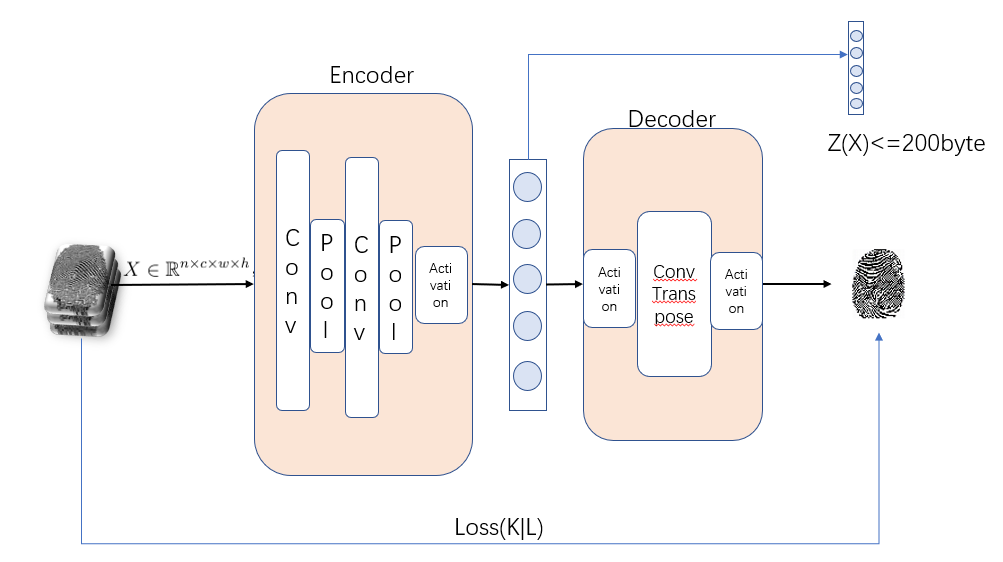
\includegraphics[width=\textwidth]{figures/model.png}
				\caption{卷积自编码器CAE模型}\label{labssel}
			\end{figure}
		其中,Conv表示全卷积,ConvTranspose表示有效值卷积,Activation表述rule激活层,Pooling表示池化层,对应的编码输入为$Z(X)<200byte$。
		
	
					将稀疏约束添加到目标函数后,自动编码器将成为稀疏的自动编码器,它考虑二值图像隐藏层的稀疏表示。 为了实现稀疏表示,本文将使用稀疏约束将重构误差最小化,加上损失函数KL散度:
								\begin{gather}
					 \mathrm{CAE}=L(X, Z)+\gamma \sum_{j=1}^{H_{D}} \mathrm{KL}\left(\rho \| \hat{\rho}_{j}\right),\\
					 \mathrm{KL}\left(\rho \| \hat{\rho}_{j}\right)=\rho \log \frac{\rho}{\hat{\rho}_{j}}+(1-\rho) \log \frac{1-\rho}{1-\hat{\rho}_{j}},
								\end{gather}
					其中γ是稀疏项的权重,$H_D$是隐藏单元的数量,ρ是稀疏性参数,通常是一个接近零的小值。$\hat{\rho}_{j}=(1 / N) \sum_{i=1}^{N} y_{j}\left(x^{(i)}\right)$是在训练集中隐藏单元j的平均激活。

在迭代修正的过程中,实验采用$Keras$自带优化器Adam函数进行迭代修正,如式~\ref{adam}~所示,其中$\beta_{1}$一般取0.9,$\beta_{2}$一般取0.999。

\begin{gather*}\label{adam}
\left\{\begin{array}{l}{m_{t}=\beta_{1} m_{t-1}+\left(1-\beta_{1}\right) \nabla_{w} f\left(w_{t}\right)} \\ {v_{t}=\beta_{2} v_{t-1}+\left(1-\beta_{2}\right) \nabla_{w} f\left(w_{t}\right)^{2}} \\ {\widehat{m}_{t}=\frac{m_{t}}{1-\beta_{1}^{t}}, \hat{v}_{t}=\frac{v_{t}}{1-\beta_{2}^{t}}} \\ {w_{t}=w_{t-1}-\eta \frac{\widehat{m}_{t}}{\sqrt{\hat{v}_{t}+\varepsilon}}}\end{array}\right.
\end{gather*}

        \subsection{实验结果及分析}
        实验训练输入样本为 400×300的指纹图片, 具体参数设置如表所示:
       \begin{table}[H]
        	\setstretch{1.4}  %设置表的行间距
        	\centering		
        	\caption{参数设置表
        	}
        	\begin{tabular}{cc|cc}
        		\toprule[1.5pt]
        		\multicolumn{1}{m{5cm}}{\centering 参数名称}
        		& \multicolumn{1}{m{2cm}}{\centering 值}
        		&        		\multicolumn{1}{m{5cm}}{\centering 参数名称}
        		& \multicolumn{1}{m{2cm}}{\centering 值}
        		\\
        		\midrule[1pt]
        		迭代次数 epoch&   2000& 吞吐量 batch & 64\\ 
        	出/入通道数 in/out& 	3/3& 编码大小 size& 200\\
        	        学习率 lr& 0.01& 偏置 $\beta_1,\beta_2$& 0.9, 0.999\\
      卷积核 $k_1,k_2,k_3$& 3,3,4& 池化层 padding& 1\\
        		\bottomrule[1.5pt]	
        	\end{tabular}
        \end{table}
    
        通过上述参数设置,计算16张指纹图片KL散度的最小值,并保存其编码程序。其迭代过程中 损失函数如下图所示:
        	\begin{figure}[H]
        	\centering
        	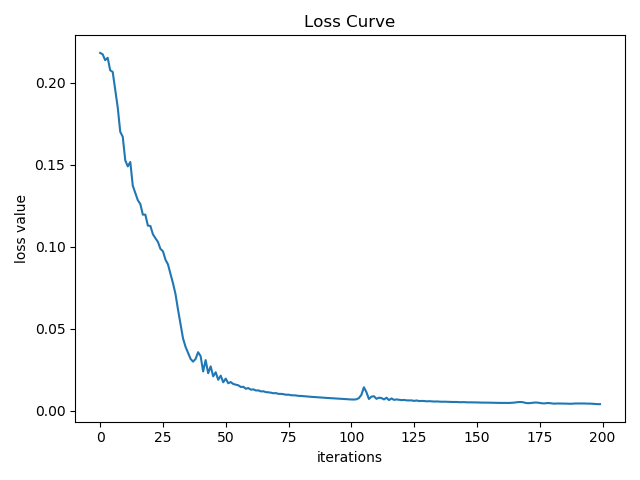
\includegraphics[width=.6\textwidth]{figures/loss.png}
        	\caption{CAE迭代过程中损失函数函数}\label{loss}
        \end{figure}
    可以看出,我们的模型在解码还原过程中,能明显逼近于真实的指纹图片,信息损失仅占0.04\%,对于传统的编码方法有明显的压缩能力。
    
    本文将指纹编码过程进行还原,得到解码图像入下图所示,可以看见CAE模型编码后再还原出的指纹图像具有高精度的还原。
        			\begin{figure}[H]	
        	\centering
        	\subfigure[指纹1过程过程]{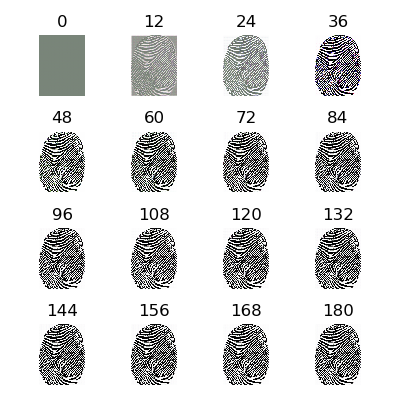
\includegraphics[height=8cm,width=7.5cm]{figures/zhiwen.png}}
        	\subfigure[指纹2解码过程]{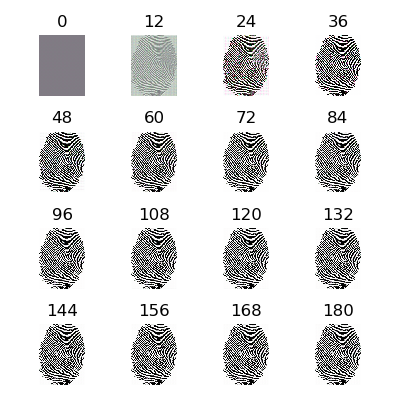
\includegraphics[height=8cm,width=7.5cm]{figures/zhiwen2.png}}
        	\caption{编码后经解码器后还原的效果图}
        	\label{zhiwen}
        \end{figure}
    
    

	\section{问题二模型的建立与求解}
		\subsection{问题描述与分析}
			问题二要求

    		其思维流程图如图~\ref{lssssct}~所示:

			\begin{figure}[H]
				\centering
				
\includegraphics[width=\textwidth]{figures/whut.jpg}
				\caption{问题二思维流程图}\label{lssssct}
			\end{figure}

		\subsection{模型的建立}
		
		\subsection{模型的求解}

        \subsection{实验结果及分析}
        
			结果如下表\ref{zhuanssssasgzai}所示:
			\begin{table}[H]
			\setstretch{1.4}  %设置表的行间距
			\centering		
			\caption{xxxxxxxxxxxxxxxxxxxxx}\label{biao1}
			\begin{tabular}{cc}
			\toprule[2pt]
				\multicolumn{1}{m{5cm}}{\centering xxxxxxx}
				& \multicolumn{1}{m{5cm}}{\centering xxxxxxx}
				\\
				\midrule[1pt]
				xxxxxxx &   909.80\\ 
				xxxxxxx & 	852.60\\ 
			\bottomrule[2pt]	
			\end{tabular}
			\end{table}
  
  			由表\ref{biao1}可知

			其各个小车的运输细节图下图所示:
			\begin{figure}[H]
				\centering
				\subfigure{
\includegraphics[height=8cm,width=7.5cm]{figures/whut.jpg}}
				\subfigure{
\includegraphics[height=8cm,width=7.5cm]{figures/whut.jpg}}
			\end{figure}	
			\begin{figure}[H]	
				\centering
				\subfigure{
\includegraphics[height=8cm,width=7.5cm]{figures/whut.jpg}}
				\subfigure{
\includegraphics[height=8cm,width=7.5cm]{figures/whut.jpg}}
				\caption{xxxxxxxxxxxxxxxxxxxxxxxxx}
				\label{fisg}
			\end{figure}

    \section{问题三模型的建立与求解}
  		\subsection{结果分析}
  
  	\section{灵敏度分析}
 
  	\section{模型的评价}
		\subsection{模型的优点}
			\begin{itemize}                                             
			\item [(1)]
			\item [(2)] 	
			\end{itemize}
		\subsection{模型的缺点}

  		\subsection{模型改进}

  
  
 
	\newpage	%换页符
	%%参考文献
	%\begin{thebibliography}{9}%宽度9
	% \setlength{\itemsep}{-2mm}
	\nocite{*}		%排版未引用的参考文献
	\begin{thebibliography}{9}%宽度9
		\bibitem{1}Davies S G. Touching Big Brother: How biometric technology will fuse flesh and machine[J]. Information Technology \& People, 2014, 7(4): 38-47.
	\bibitem{2}Moses K R, Higgins P, McCabe M, et al. Automated fingerprint identification system (AFIS)[J]. Scientific Working Group on Friction Ridge Analysis Study and Technology and National institute of Justice (eds.) SWGFAST-The fingerprint sourcebook, 2011: 1-33.
	\bibitem{3}Dror I E, Wertheim K, Fraser‐Mackenzie P, et al. The impact of human–technology cooperation and distributed cognition in forensic science: biasing effects of AFIS contextual information on human experts[J]. Journal of forensic sciences, 2012, 57(2): 343-352.
	\bibitem{4}Simonyan K, Zisserman A. Very deep convolutional networks for large-scale image recognition[J]. arXiv preprint arXiv:1409.1556, 2014.
	\bibitem{5}
	\end{thebibliography}

	\newpage
	%附录
	\appendix %%附录
	\section{数据可视化的实现}
		\subsection*{第一问画图--python源代码}
			\begin{lstlisting}[language=python]
			
			\end{lstlisting}
			
		\subsection*{第二问画图--python源代码}
			\lstinputlisting[language={python},numbers=left,numberstyle=\tiny,
			rulesepcolor=\color{red!20!green!20!blue!20},  
			keywordstyle=\color{blue!70!black},  
			commentstyle=\color{blue!90!},  
			basicstyle=\ttfamily] {./code/demo.py}

\end{document}